% 1977 年山东B卷第 7 题：平行四边形 ABCD，M 为大边 AB 的中点，连接 MD、MC（按源卷第 3 页布局）
% D 左上、C 右上、A 左下、M 在 AB 中点、B 右下
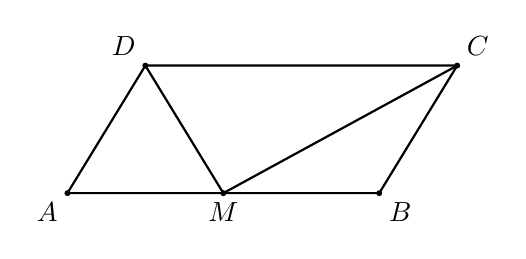
\begin{tikzpicture}[scale=0.9]
  \coordinate (A) at (0,0);
  \coordinate (M) at (2.2,0);
  \coordinate (B) at (4.4,0);
  \coordinate (D) at (1.1,1.8);
  \coordinate (C) at (5.5,1.8);
  \draw[thick] (A)--(B)--(C)--(D)--cycle;
  \draw[thick] (D)--(M);
  \draw[thick] (M)--(C);
  \fill (A) circle (1.2pt) node[below left] {$A$};
  \fill (M) circle (1.2pt) node[below] {$M$};
  \fill (B) circle (1.2pt) node[below right] {$B$};
  \fill (D) circle (1.2pt) node[above left] {$D$};
  \fill (C) circle (1.2pt) node[above right] {$C$};
\end{tikzpicture}
